\section {Introduction}

The S12XEMU is a timed system level simulator of the Freescale processor MC9S12XDP512. It is able to load, disassemble and run ELF as well as S-Format binary. It is written to run under linux platform and hence provide the best performance. It is usable also under win32 by means of mingw32 and some loose of speed.\\
\\
The main features of the S12XEMU simulator are:
\begin{itemize}\addtolength{\itemsep}{-0.40\baselineskip}
\item Load, disassemble and run of CPU12/CPU12X binary
\item Software debugging
\item Trace generation
\item Usable in co-simulation context using systemc/TLM2 communication interfaces
\item Fully configurable behavior (frequency, max-instructions, debug, trace, logs, etc.)
\end{itemize}

\section {Simulated configuration}

The simulator include the following components:
\begin{itemize}\addtolength{\itemsep}{-0.40\baselineskip}
\item Full CPU12X instruction set simulator
\item Memory Mapping Control (S12XMMCV2)
\item Simple router to memory and peripherals
\item Simple router to global memory and external addressing space
\item 64 Ko local memory
\item 8 Mo global memory
\item Analog-to-Digital Converter ATD10B16CV4 and S12ATD10B8CV3
\item Clock and Reset Generator
\item Pulse-Width Modulator (S12PWM8B8CV1)
\item Interrupt (S12XINTV1)
\end{itemize}

The simulator uses the following services:
\begin{itemize}\addtolength{\itemsep}{-0.40\baselineskip}
\item ELF loader
\item S-Record loader
\item GDB Server
\item Inline debugger
\item SystemC Time
\item Host Time
\end{itemize}

\begin {figure}[h]
	\centering
		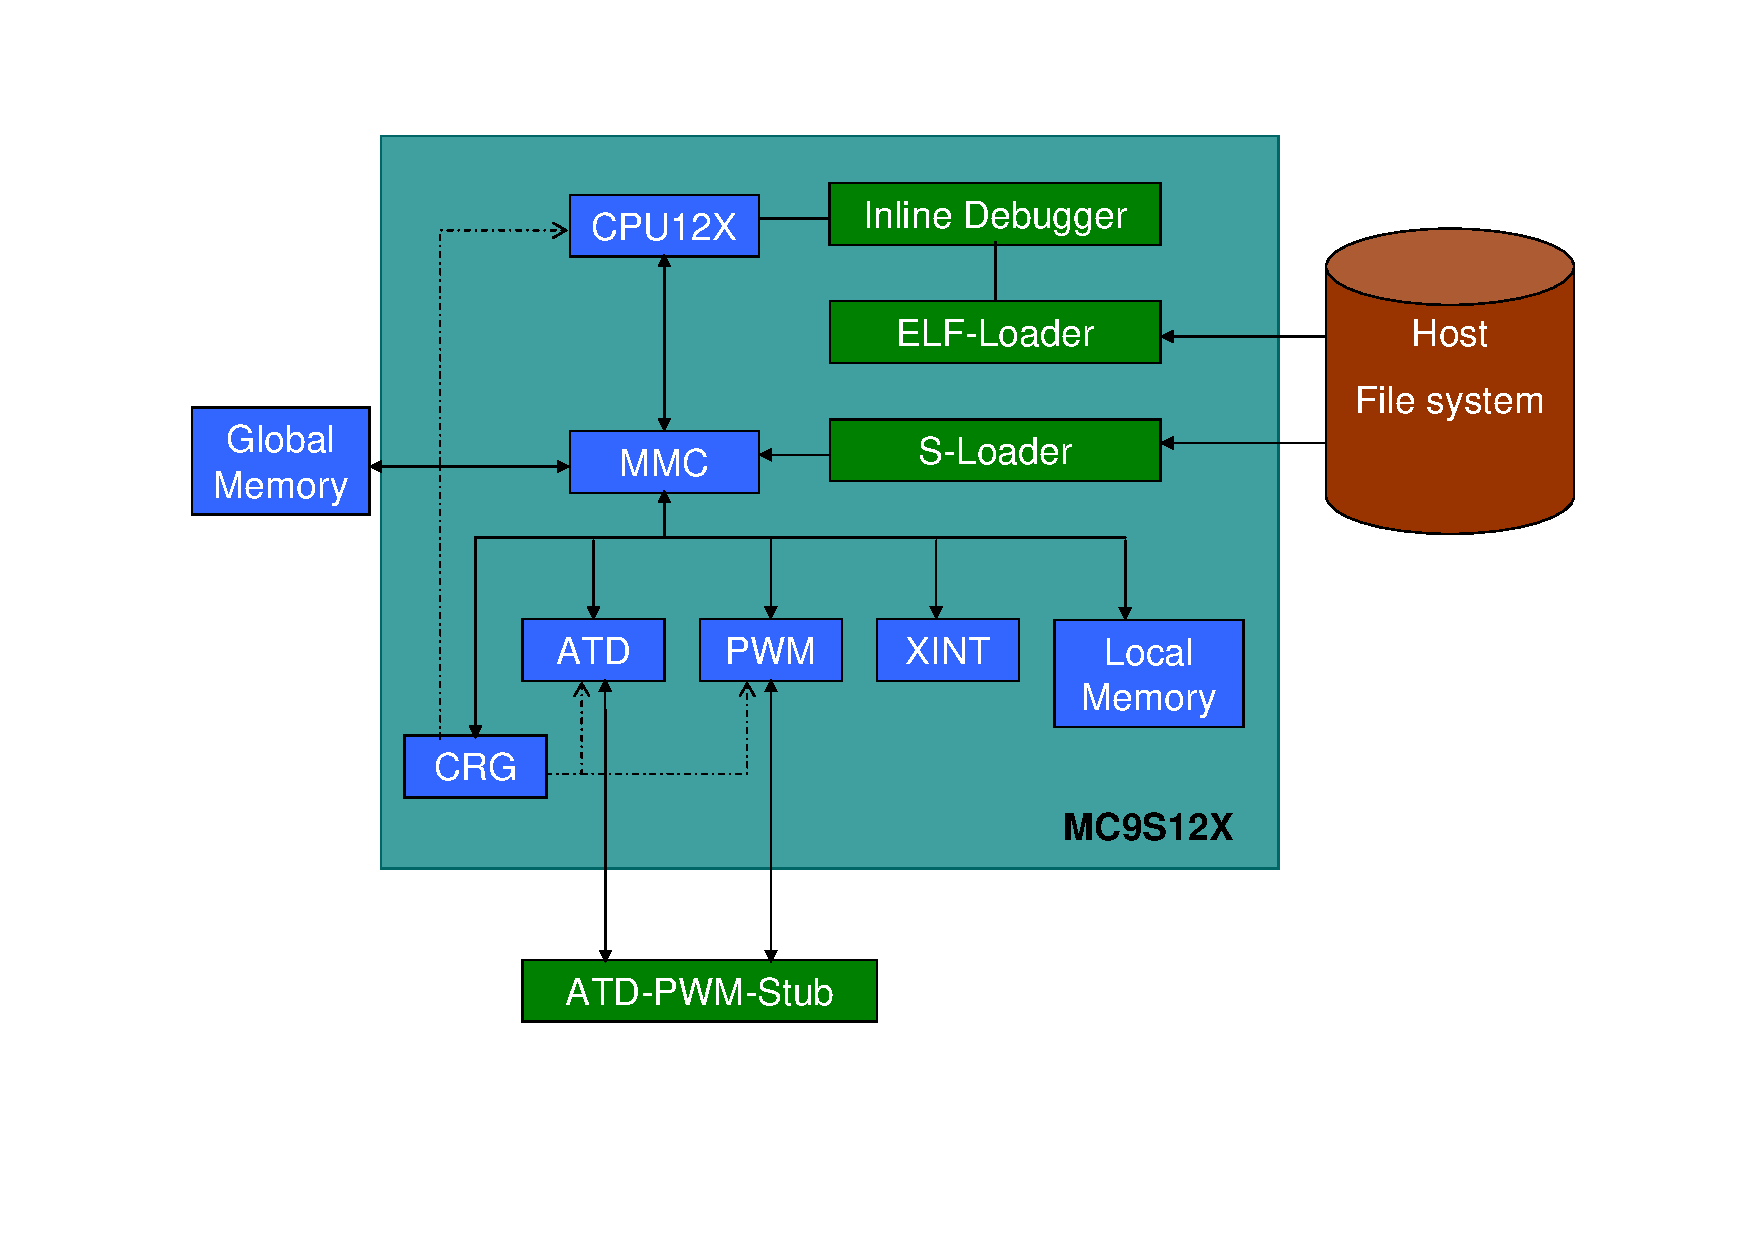
\includegraphics[width=1\textwidth]{mc9s12xdp512/mc9s12xdp512_schema.pdf}
	\caption {mc9s12x configuration.}
	\label {fig:mc9s12xdp512}
\end {figure}

\section{Using the simulator}

Usage: \texttt{s12xemu [<options>] <program> [program arguments]}
\\

Options:
\begin{itemize}

\item Starts the inline debugger

\texttt{--inline-debugger}
\\
\texttt{-d}

\item Virtual Platform configuration file

\texttt{--parameters-filename <xml file>}
\\
\texttt{-p <xml file>}

\item Get the virtual Platform default configuration xml file (you can use it to create your own configuration). This option can be used with -p to get a new configuration file with existing variables from another file

\texttt{--extract-parameters-filename <xml file>}
\\
\texttt{-x <xml file>}

\item Start a gdb server

\texttt{--gdb-server <TCP port>}
\\
\texttt{-g <TCP port>}

\item Uses $<arch file>$ as architecture description file for GDB server

\texttt{--gdb-server-arch-file <arch file>}
\\
\texttt{-a  <arch file>}

\item Set the memory map modele to use for decoding addresses

\texttt{-c <mode>}
\\
\texttt{--compiler-memory-modele <mode>}
\\
\\
            0: banked modele (default)\\
            1: linear modele (recommended by Motorola/Freescale)\\
            2: gnu/gcc modele\\

\item Program symbols file. Used for debbug purpose when loading an S19-File

\texttt{-s <symbol filename>}
\\
\texttt{--symbol-filename <symbol filename>}

\item Force the ELF loader to use segment virtual address instead os segment physical address

\texttt{-f}
\\
\texttt{--force-use-virtual-address}

\item Displaying the integrated help

\texttt{--help}
\\
\texttt{-h}

\end{itemize}


